\documentclass[11pt]{article}
\usepackage[ugly]{thesis}

\definecolor{TODO}{HTML}{0000BB}

\begin{document}
\pagestyle{plain}
\title{\rmfamily\normalfont\spacedallcaps{Decision
Problems in Invertible Automata}} \author{\spacedlowsmallcaps{Evan
Bergeron \& Klaus Sutner}} \date{May 5, 2017}

\maketitle

\begin{abstract}
  We consider a variety of decision problems in groups and semigroups
  induced by invertible Mealy machines. Notably, we present proof
  that, in the Abelian case, the emutomorphism membership problem in
  decidable in these semigroups. In addition, we prove undecidability
  of a Knapsack variant. A discussion of iteration and orbit
  rationality follows.
\end{abstract}
% \newpage

\tableofcontents
% \newpage

\section{Introduction}
The word problem is a classic group-theoretic decision problem. Given
a finitely generated group $G$, and a word $w$ over the generators
(and their inverses), the word problem asks ``is $w \in G$.'' The word
problem is known to be undecidable in surprisingly small classes of
groups - see \cite{Cain09:auto_sg} and \cite{Cain09:dec_prob} for background.

The invertible Mealy machines we consider here give rise to a class of
semigroups (and sometimes groups) for which the word problem is
decidable. The computability picture here is rather nuanced,
however. Similarly important decision problems, among them the
conjugacy problem, and the isomorphism problem are known to be
undecidable - see \cite{sunic:conj} and TODO for details.

We present proof that, for the Abelian case, automorphism membership
testing is decidable in this class of semigroups.

Invertible automata have recently been usefully applied the group
theory. A classic result here is Grigorchuk's group of intermediate
growth, generated by the 5 state invertible machine shown in figure 1.

\begin{figure}
\begin{center}
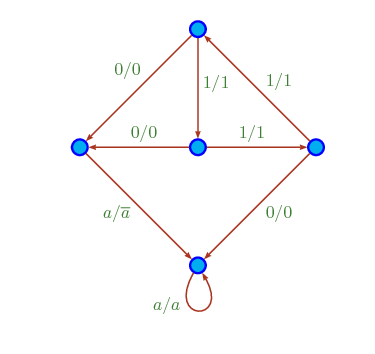
\includegraphics[scale=0.5]{figures/grigorchuk}
\end{center}
\caption{Grigorchuk's 5 state machine}
\end{figure}
\section{Background}
An \defn{automaton} is a formally a triple $(Q, \Sigma, \delta)$,
where $Q$ is some finite state set, $\Sigma$ is a finite alphabet of
\defn{symbols}, and $\delta$ is a transformation on $Q \times \Sigma$.
Automata are typically viewed as directed graphs with vertex set $Q$
and an edge labeled $x \mid y$ between $u, v$ if $(u, x)\delta = (v, y)$.

\begin{center}
\begin{tikzpicture}[
        > = stealth, % arrow head style
        shorten > = 1pt, % don't touch arrow head to node
        auto,
        node distance = 2.5cm, % distance between nodes
        semithick % line style
    ]
    \tikzstyle{every state}=[
        draw = black,
        thick,
        fill = white,
        minimum size = 4mm
    ]
    \node[state] (start) {$u$};
    \node[state] (halt) [right of=start] {$v$};
    \path[->] (start) edge node {$x \mid y$} (halt);
\end{tikzpicture}
\end{center}

One interprets this as if $\A$ is in state $u$ and reads symbol $x$,
then $\A$ transitions to state $v$ and outputs symbol $y$. A
computation within $\A$ may then start at some state $q_0$, and on
input $\alpha_0 \alpha_1 \ldots \alpha_k$, output
$\beta_0 \beta_1 \ldots \beta_k$, where
$(q_i, \beta_i) = (q_{i-1}, \alpha_i)\delta$ for all $i = 0\ldots k$.

As in the above case, where $\delta$ outputs exactly one character forbe
every transition, we call the automaton $\A$ \defn{synchronous}. An
automaton is called \defn{invertible} when every state in $Q$ has some
bijection $\pi$ on $\Sigma$ such that $(u, x)\delta = (v, \pi(x))$. A
state in $\A$ is a \defn{copy state} if $\pi$ is the identity
permutation and is a \defn{toggle state} otherwise. The present paper
is concerned only with invertible, synchronous automata.

\subsection{Actions on the infinite tree}

We may identify the set $\Sigma^*$ with an infinite, regular tree of
degree $|\Sigma|$. The root is labelled with the empty string
$\epsilon$, and a vertex labelled $w$ has the child $wa$ for each
$a \in \Sigma$. Out of convenience, we will frequently conflate a
vertex with its label.

% TODO make this less ugly
\begin{center}
\begin{tikzpicture}[
        > = stealth, % arrow head style
        shorten > = 1pt, % don't touch arrow head to node
        auto,
        node distance = 1.5cm, % distance between nodes
        semithick % line style
    ]
    \tikzstyle{every state}=[
        draw = black,
        thick,
        fill = white,
        minimum size = 3mm
    ]
    \node[state] (root) {$\epsilon$};
    \node[state] (s0) [below left  of=root] {$0$};
    \node[state] (s1) [below right of=root] {$1$};
    \node[state] (s00) [below left  of=s0] {$00$};
    \node[state] (s01) [below right=0.56cm and 0.1cm of s0] {$01$};
    \node[state] (s10) [below left=0.56cm and 0.1cm of s1] {$10$};
    \node[state] (s11) [below right of=s1] {$11$};
    \path[->] (root) edge node {} (s0);
    \path[->] (root) edge node {} (s1);
    \path[->] (s0) edge node {} (s00);
    \path[->] (s0) edge node {} (s01);
    \path[->] (s1) edge node {} (s10);
    \path[->] (s1) edge node {} (s11);
\end{tikzpicture}
\end{center}

Each state $q \in Q$ acts on the corresponding tree, sending vertex
$w$ to $wq$. Moreover, if $\alpha \alpha' q = \beta \beta'$, then
$\alpha q = \beta$, for any
$\alpha, \alpha', \beta, \beta' \in \Sigma^*$. Which is to say, $q$'s
action on the tree is an adjacency-preserving map and is thus an
endomorphism on the tree. Since $\A$ is synchronous, $q$ is
length-preserving, and thus preserves levels of the tree (and thus is
an automorphism of the tree).

% TODO to talk about faithful actions, need some wreath recursion
% background. Maybe move this generalization after the wreath
% recursion part?
We extend the action of $Q$ on $\Sigma^*$ to words $q = q_1\ldots q_n$
over $Q^+$ by \[ wq = (\ldots((w q_1) q_2)\ldots q_n). \]

This computation corresponds with running $\A$ starting at state $q_1$,
then taking that output and running it through the machine starting at
state $q_2$, and so on. We adopt the convention of applying functions
from the right here. In this way, function composition corresponds
naturally with string concatenation.

So there is a natural homomorphism
$\phi : Q^+ \rightarrow \operatorname{Aut}B^*$, where
$\operatorname{Aut}B^*$ denotes the semigroup of automorphisms of the
tree $B^*$. We denote the image of $\phi$ by $\Sigma(\A)$.

\subsection*{Semigroup theory}

A \defn{semigroup} is a set $S$ paired with a binary operation
$f : S \times S \rightarrow S$ such that $S$ is closed under $f$ and
$f$ is associative over $S$. Any set of endofunctions forms a
semigroup under composition.

A semigroup is called \defn{Abelian} when its corresponding binary
operation is commutative.

For an automaton $\A$, we denote by $S(\A)$ the semigroup generated by
$Q$ under composition. $\A$ is said to be \defn{commutative} or
\defn{Abelian} when $S(\A)$ is Abelian. We write $G(\A)$ for the group
generated by the elements of $Q$ and their inverses.

One may also speak about $S(\A)$ and $G(\A)$ without explicit reference
to an automaton $\A$. As such, we call a semigroup $S$ an
\defn{automaton semigroup} if there is some automaton $\A$ with
$S \simeq \Sigma(\A)$.
% TODO expand on this
\defn{Automaton groups} $G$ are similarly defined.

\subsection*{Wreath Recursions}
Any automorphism $f$ of $\Sigma^*$ can be written in the recursive form:
\[ f = (f_{\alpha_1}, f_{\alpha_2}, \ldots, f_{\alpha_n})\tau \] where
$n = |\Sigma|$ and each $f_\alpha$ is an automorphism of a subtree of
the root. Here, $\tau$ is some permutation on $\Sigma$. In the case
where $\Sigma = \{0, 1\}$, we have $f = (f_0, f_1)\sigma$ where
$\sigma$ denotes transposition. If $f = (f_0, f_1)\sigma$, $f$ is said
to be \defn{odd}. If $f = (f_0, f_1)$, f is said to be
\defn{even}. That is to say, automorphisms may be classified as even
or odd depending on their action on the first level of the tree. The
set of even automorphisms form a subgroup $H$ of index 2 in
$G(\A)$. Further, the residuation maps are group homomorphisms when
restricted to $H$.

The automorphism semigroup of $\Sigma^*$ decomposes into a recursive
wreath product
\[
  \operatorname{Aut}B^* = \operatorname{Aut}B^* \wr \tau_\Sigma
\]
where $\tau_\Sigma$ is the tranformation semigroup on $\Sigma$. Which
is to say,
% TODO put the curly underbrace for $n$ times underneath
\[
  \operatorname{Aut}B^* = (\operatorname{Aut}B^* \times \ldots \times
  \operatorname{Aut}B^* ) \rtimes \tau_\Sigma
\]

We have \emph{residuation maps} $\partial_a : S(\A) \rightarrow S(\A)$
that map $f = (f_0, f_1)\sigma$ to $f_a$, and a \emph{parity map}
$\textsf{par}$ such that $\textsf{par}(f) = \sigma$.

Note that a subgroup $G$ of $\operatorname{Aut}(2^*)$ need not be
closed under residuation; if it is, we call it \emph{self-similar} or
\emph{state-closed}. In this case, the wreath characterization in the
full automorphism group carriers over and we have
$G \cong (G \times G) \rtimes \tau_{\textbf{2}}$.

% TODO running example
% TODO an example here would be very very useful

% TODO
% Cosets thing

\section{Decision Problems}

Automaton semigroups exhibit many interesting and nuanced
computability properties. While it is an easy result that the
\decprob{word problem} is solvable in such semigroups, similar
group-theoretic problems such as the \decprob{conjugacy problem} and
\decprob{finiteness problem} have been shown to be undecidable
(see \cite{sunic:conj}, and \cite{gillibert:finite}, respectively).

Various other semigroup theoretic decision problems have recently been
considered for small classes of semigroups by Cain in
\cite{Cain09:dec_prob}. We consider a subset of his distinguished
properties in the automaton semigroup case here.

% TODO finitely generated and other background

\subsection{\decprob{IsAbelian} is polynomial time}

For a binary invertible automaton $\A$, define the \emph{gap} of an
automorphism $f \in G(\A)$ to be
$\gamma_f = (\partial_0 f)(\partial_1 f)^{-1}$.

The following result is adapted from \cite{okano:thesis}.

% TODO omg this typesetting
\textbf{Lemma}. $\A$ is Abelian if and only if all even automorphisms
in $S(\A)$ have gap $I$ and odd automorphisms have constant gap.

\begin{proof}
Suppose $\A$ is Abelian; so $fg = gf$ for all $f$, $g$ in $S(\A)$.
If $f$ and $g$ are both odd, simply residuate both sides to get
\[
  (\partial_a f)(\partial_{\bar{a}}g) =
  \partial_a (fg) =
  (\partial_a gf) =
  (\partial_a g)(\partial_{\bar{a}}f)
\]
which yields $\gamma_f = \gamma_g$. If $f$ is even and $g$ odd, without loss of generality, we have
\[
  (\partial_0f)(\partial_0 g) = 
  \partial_0(fg) =
  \partial_0(gf) =
  (\partial_0g)(\partial_1 f)
\]
which, with algebraic manipulation, yields $\gamma_f = I$.

Conversely, first suppose $f$ and $g$ are both odd. Then
$fg = (\partial_0 f \partial_1 g, \partial_1 f \partial_0 g)$ and
$gf = (\partial_0 g \partial_1 f, \partial_1 g \partial_0 f)$. Since
$\gamma_f = \gamma_g$, these wreath recursions are the same. If $f$ is
even and $g$ odd, TODO

If $f$ and $g$ are both even, the claim follows by induction.
\end{proof}

{\color{TODO}
So it suffices to verify that each toggle state obeys this.

Since these transducers are synchronous (output exactly one character
per transition), we can build a DFA that recognizes the input-output
relation of some fixed starting state. Take some $s$ this start
state. Then build a DFA over the alphabet $\Sigma \times \Sigma$ with
transitions simulating the behavior of the transducer starting at
$s$. This DFA is called the \textit{acceptor of $\A$ at $s$}.

An automaton semigroup $S(\A)$ has a presentation with generators
corresponding to the states of $\A$. Thinking of elements of $S(\A)$ as
words over this generator alphabet, we see that the state set of $\A$
is precisely the words of length 1. We can build an automaton whose
state set is the set of all length 2 words as follows:

If $\A = (Q, \Sigma, \delta)$, the product automaton $\A \times \A$ has
state set $Q\times Q$ with transition function
$\partial_a (s_1, s_2) = (\partial_a s_1, \partial_{a s_1} s_2)$. We
can see by induction that each state $(s_1, s_2)$ corresponds to the
word $s_1 s_2 \in S(\A)$.

Remember that
$(\partial_1 \underline{t}) = (\partial_0 \underline{t})\Theta_\A$. So
then we have
$(\partial_1 \underline{t})(\partial_0 \underline{t})^{-1} =
\Theta_\A$. (This is straight from Okano's thesis, I think this
expression is better written as
$(\partial_0 \underline{t})^{-1}(\partial_1 \underline{t})= \Theta_\A$
- it seems more consistent with function-application-from-the-right).

Anyway, $\Theta_\A = (\partial_1 \underline{t})(\partial_0 \underline{t})^{-1} = (\partial_1 \underline{t})(\partial_1 \underline{t^{-1}})$, where $t^{-1}$ lies in the inverse automaton for $\A$. So then build for each toggle state the following: $(\A\times \A^{-1})(\partial_1 \underline{t}, \partial_1 \underline{t^{-1}})$. Note that the language of this automaton is $\{ x : y \mid y = x(\partial_1 \underline{t})(\partial_0 \underline{t})^{-1}\}$. It suffices to then verify that all of these constructed DFAs are equivalent, which can be done via Hopcroft's minimization algorithm.

So to summarize algorithmically: take the input automaton $\A$. Build
it's inverse automaton $\A^{-1}$. Construct the product automaton
$\A\times \A^{-1}$. Then for each toggle state $t_i$ of $\A$, take the
state $s_i = (\partial_1 t_i, \partial_1 t_i^{-1})$ in
$\A\times \A^{-1}$ and construct the DFA $(\A\times \A^{-1})(s_i)$. Verify
all the constructed DFAs are equivalent.

% Interestingly, note that this approach leads to (new?) proof of the
% following claim:

This product automaton construction also gives us that the word
problem for automaton semigroups is decidable.
} % ENDTODO

\subsection{Automorphism \decprob{Membership}}

This section considers the subsemigroup $G(\A)$ of
$\operatorname{Aut}2^*$ generated by the associated autormophisms of
an invertible binary transducer. We assume minimality throughout this
section.

We provide proof that the automorphism membership question is
decidable in the Abelian case, and discuss partial work toward the
general case. Some necessary background from
\cite{NekrashevychSidki04:automorphisms} is outlined below.

\subsubsection{Linear algebraic background}

% TODO this is disgusting typesetting.
\begin{theorem}
If $\A$ is a commutative automaton, then $G(\A)$ is
isomorphic to either a finite Boolean group or to $\Z^m$ for some
$m \geq 1$. In the latter case, there is an isomorphism
$\phi : G(\A) \rightarrow \Z^m$ satisfying the following recursion
\[
  \phi^{-1}(v) =
  \begin{cases}
    (\phi^{-1}(A\cdot v), \phi^{-1}(A \cdot v)) & \text{if $\phi^{-1}$ is even}\\
    (\phi^{-1}(A\cdot v - r), \phi^{-1}(A \cdot v + r)) &
    \text{otherwise}
  \end{cases}
\]
\end{theorem}

We call the matrix $A$ above the \defn{residual matrix} of $A$. The
vector $r$ is referred to as the \defn{residual vector}.

We have the following properties of $A$:

% TODO don't conflate the automaton A with the matrix A
\begin{theorem}
If $G(A) \cong \Z^m$ and $A$ is its associated
residual matrix, $A$ satisfies the following properties:
\begin{enumerate}
\item $A$ is contracting; its spectral radius is less than 1
\item $A$ is 1/2-integral, meaning that $A^{-1}$ is a subgroup of
  index 2 in $\Z^m$. Therefore $A$ be represented as TODO where all
  $a_{i,j}$ are integers.
\item The characteristic polynomial $\chi_A(x)$ is irreducible over
  $\Q$ and has the form
  \[ \chi_A(x) = x^m + \frac{1}{2}g(x) \] for some $g \in \Z[x]$ of
  degree $m-1$. In particular, the constant term is $+-\frac{1}{2}$.
\item $A$ is invertible and the characteristic polynomial
  $\chi_{A^{-1}}(x)$ is integral and irreducible over $\Q$. From
  property 2, Laplace expansion yields that $A^{-1}$ is an integral
  matrix that is similar to the companion matrix of $\chi_{A^{-1}}(x)$
  over $\Q$.
\end{enumerate}
\end{theorem}

Latimer and MacDuffee proved the following theorem in TODO

\begin{theorem}
  If $p(x) \in \Z[x]$ is monic and irreducible, the $GL(m, \Z)$
  similarity classes of integral matrices whose characteristic
  polynomial coincides with $p(x)$ is in one-to-one correspondance
  with ideal classes of the ring $\Z[\theta]$, where $\theta$ is any
  root of $p(x)$.
\end{theorem}

Property 1 of the first theorem provides a bound on the coefficients
of $\chi_A(x)$. When combined with property 4 and the above theorem,
it can be shown that, for fixed $m$, there exist only finitely many
possibilities of $A$, up to $GL(m, \Z)$ similarity.

TODO complete automata etc.

\textbf{Example} The following automata represent the subautomata of the complete automaton generated with residual matrix
\[
  A = \begin{bmatrix}
    -1 &1\\
    -\frac{1}{2} & 0
    \end{bmatrix}
\]
and residual vector $r = TODO$.

% TODO finish these diagrams, make this one not ugly
\begin{center}
\begin{tikzpicture}[
        > = stealth, % arrow head style
        shorten > = 1pt, % don't touch arrow head to node
        auto,
        node distance = 2.5cm, % distance between nodes
        semithick % line style
    ]
    \tikzstyle{every state}=[
        draw = black,
        thick,
        fill = white,
        minimum size = 4mm
    ]
    \node[state] (zero) {};
    \node[state] (two) [below right of=zero] {};
    \node[state] (one) [below left of=zero] {};
    \path[->] (zero) edge node {} (two);
    \path[->] (zero) edge node {} (one);
    \path[->] (two) edge node {} (one);
    \path[->] (one) edge node {} (zero);
\end{tikzpicture}
\end{center}

\subsubsection{\decprob{Membership} is decidable in the Abelian case}


% TODO definitions of principal automaton, complete automaton, etc

{\color{TODO}
Given an invertible automaton $\A$ and a principal Abelian automaton
$\B$, we determine if $f = \A(p)$ is in the semigroup generated by $\B$.

Thus one needs to check if there is some product automaton
\[
  D = \B_{p_1} \times \B_{p_2} \times \ldots \times \B_{p_n}
\]
that implements $f$. We have no computable bound on $n$, so a priori
this merely semidecidable.

Now consider the complete automaton $C$ for $\B$, and let $g$ be the
automorphism defined by $D$. After minimization, $D$ produces a
subautomaton of $C$ tat consists of a ``transient part'' and a copy of
$\B$ (there may be SCCs in the transient part, but they are not
subautomata). Hence, there is some word $w$ such that $\partial_w g$
is just a single state in the copy of $\B$; also, $w$ can be found
effectively\footnote{TODO}. In fact, for all $u$, there is a $w$ such
that $\partial_{ww}g$ is atomic. Essentially this just means that $g$
is strongly tame.

We may safely assume that $\A$ is minimal. Then is looks like $\A$ has
to have $\B$ as a subautomaton to satisfy this ultimate atomicity
condition, plus a transient part sitting on of $\B$. It should be
decidable if things match up.

If $\B$ is not principal, there are multiple subautomata of $C$ to
content with, but that should not make a major difference. Ditto if
$\B$ is just a random subautomaton of $C$.

% TODO
% If same A and r, just identity check.
% If same A, rdifferent r - nontrivial now.
%   - Just a linear subspace problem.
%   - We can assume we have the info up front
%   - Answer is no qne-way and yes the other (bowtie and A32)
% Different A:
%   - Charpoly changes here. Tell you about the identities.
%   - TODO
%   - just write out the equations for the thing you're testing
%
% TODO - come up with two automata with separate A, r, A', r'
%        but there's a function in one machine that can be simulated in the
%        other.
}

\subsubsection{\decprob{Membership} is open in the general case}

\subsection{\decprob{IsGroup}}
\subsubsection{\decprob{IsGroup} is decidable in the Abelian case}
\subsubsection{\decprob{IsGroup} is open in the general case}

\subsection{\decprob{Knapsack} is undecidable for automaton semigroups}
We follow a proof strategy similar to \cite{Konig15:knapsack}.

We define the \decprob{Knapsack Problem} as follows: given as input
generators $g_1 \ldots g_k$ and a target semigroup element $g$, do there
exist natural numbers $a_1\ldots a_k$ such that
\[ g_1^{a_1} \cdots g_k^{a_K} = g \]


% TODO reducing "to"?
We prove that this problem is undecidable for automaton semigroups by
reducing from Hilbert's tenth problem.

We define the decision problem \decprob{Hilbert} as following: ``given
a polynomial over the integers and an integer $a$, do there exist
values of the arguments to the polynomial such that the polynomial
evaluated at this point is equal to $a$?'' It is known that there
exist polynomials for which this problem is undecidable.

\begin{theorem}
  \decprob{Knapsack} is undecidable in the class of automaton semigroups.
\end{theorem}

{\color{TODO}
We can expand this polynomial into a system of equations - think of a
codegen step in a compiler. Each step is either an addition or a
multiplication. We can take the terms with negative coefficients and
move them to the other side of the equation, so we now have the
equality of two different polynomials, each with positive
coefficients. We can also choose to only substitute in natural numbers
as arguments, by some trick that I don't know. So then we have systems
of equations over the natural numbers.

We can turn each equation into a formulation of the Knapsack problem
for automaton semigroups. It's known that the Heisenberg semigroup is
an automaton group, and there's some equation over the elements of
$H_3$ for multiplication. Same for addition in the natural
numbers. Then we just take the direct product of these groups (the
class of automaton semigroups is closed under direct product). So this
polynomial is equal to $a$ if and only if there exist $a_1 \ldots a_n$
such that each of the individual elements of the direct product
vectors are equal.

We reduce from Hilbert's tenth problem, over natural numbers. Fix a
polynomial $P(x_1, \ldots x_n)$ such that the question ``is there a
solution to $P(x_1, \ldots x_n) = a$'' is undecidable.

% \begin{algorithm}
% \begin{algorithmic}[1]
% \Procedure{HilbertsTenth}{}
% \EndProcedure
% \end{algorithmic}
% \end{algorithm}

% \begin{verbatim}
% def hilbertsTenth(a):
%   # P fixed
%   P_plus = all positive terms of P
%   P_neg = all negative terms of P
% \end{verbatim}

Take $P$ and separate it into $P_+$ and $P_-$, the positive and
negative parts of $P$. Consider the equation $P_+ = P_-$.
} % ENDTODO

\subsection{A monoid with decidable \decprob{Word Problem} and undecidable \decprob{IsGroup}} 

% TODO monoid definition
We establish the existence of a monoid with decidable
$\decprob{Word Problem}$, but undecidable $\decprob{IsGroup}$. We may
take this result as an intermediate step toward the decidability of
the $\decprob{IsGroup}$ problem for automaton semigroups.

\subsubsection*{Preliminaries}
Here we take a \defn{Turing machine} to be a 6-tuple,
$(Q, \Sigma, \Gamma, \delta, q_0, q_{accept}, q_{reject})$, where $Q$,
$\Sigma$, $\Gamma$ are all finite sets.
$\delta : Q \times \Sigma \rightarrow Q\times \Gamma \times \{L,S,R\}$
is the transition function, $Q$ is the state set, $\Sigma$ is the
input alphabet, $\Gamma \supseteq \Sigma$ is the tape alphabet, $b$ is
some blank symbol, with $b \in \Gamma - \Sigma$, $q_{accept}$ is the
unique accepting final state, and $q_{reject}$ the single rejecting
final state.

We further define a Turing machine \defn{configuration} to be a triple
$(u, q, v) \in \Gamma^* \times Q \times \Gamma^*$. Here, $u$ denotes
the tape contents to the left of the tapehead, $q$ is the current
state, and $v$ begins at the tapehead and extends to the right.

A configuation $C$ for a TM $M$ is said to \defn{yield} configuration
$C'$ if $M$ can step directly from $C$ to $C'$.

For a Turing machine $M$, take $C_M$ to be the set of all valid
configurations of $M$. Then define $CG_M$ to be the graph $(C_M, E)$,
where $(u,v) \in E$ if and only if $u$ yields $v$ in $M$. Define
% TODO define \mathcal{T} to be the set of all TMs
\[
  \textsf{canon}(M, w) : \mathcal{T} \times \Sigma^*
      \rightarrow
       C_M^*\cup C_M^\omega
\]
to be the function that maps input $w$ to the sequence of
configurations $M$ takes on while computing over
$w$. $\textsf{canon}(M, w)$ will be a finite sequence if and only if
$M$ halts on $w$. We call $\textsf{canon}(M, w)$ the \defn{canonical
 computation of $M$ on $w$}.

Certainly, not every configuration in $C_M$ will be along the sequence
$\textsf{canon}(M,w)$. Which is to say, there are unreachable
configurations.

Informally, a \defn{self-verifying Turing machine} $S$ is one that, at
every step, verifies that the current configuration lies upon the
canonical computation. If $S$ finds that this is not the case, $S$
immediately rejects. Otherwise, the computation steps forward a single
step.

In the configuration graph $CG_S$, there is a path extending from each
valid starting configuration $(\epsilon, q_0, w)$ for $w \in \Sigma^*$. The remaining states form an infinite star graph with $q_{reject}$ as the center.

\textit{Claim:} There is a computable\footnote{TODO is actually
  primitive recursive} function $\textsf{sv}$ that maps Turing
machines to equivalent self-verifying Turing machines.

Speaking informally, as the canonical computation proceeds, a program
counter is kept - perhaps to the left of the tapehead. After every
step, the Turing machine will examine what ``time step'' the
computation is currently sitting in. It will perform the canonical
computation for the first $n$ steps. If it does not wind up where it's
configuration says it is, it transitions to the death
state. Otherwise, it continues.

In the interest of reader intuition, we expound upon a couple of
implementation details here. For further reading, see
\cite{davis:note_utm}, \cite{davis:defn_utm}, and
\cite{shepherdson:machine_config}.

TODO rough sketch of implementation details.

\subsubsection*{The submonoid in question}
Define the Turing machine $M = (Q, \Sigma, \Gamma, \delta, q_0, F)$ to
operate only on the blank tape; for all $s \in \Sigma$,
$\delta(q, s) = (q_{reject}, b, S)$

% TODO need to make the Turing machine maintain a counter, right?

Then take the ambient Abelian group $G_M = (C_M, \cdot)$ whose carrier
set is all configurations of $M$. For $c$, $c'$ in $G_M$, we have
$c = c'$ if and only if $c$ yields $c'$.

\textit{Claim:} $G_{\textsf{sv}(M)}$ has a decidable word problem.

For every word $w$ in $G_{\textsf{sv}(M)}$, there exist nonnegative
integers $a$, $r$ such that $w = q_{accept}^a q_{reject}^r$. Further,
we may compute $a$ and $b$. Recall that $\textsf{sv}(M)$ maintains a
program counter $p$ to the left of the input. So we may simply run $M$
for the first $p$ steps and then check for configuration equality.

So then given two words $w_1$, $w_2$ in $G_{\textsf{sv}(M)}$, simply
compute $a_1$, $r_1$, $a_2$, $r_2$. Return true if and only if $a_1 = a_2$ and $r_1 = r_2$.

\textit{Claim:} If $s$ is the start configuration of the Turing
machine, it is undecidable whether $\langle s \rangle$ is a group.

% TODO formalize
It is well known that the following language is undecidable
\[
  \decprob{halts} = \{\langle M \rangle \mid \text{TM $M$ halts on
    $\epsilon$} \}
\]
and so we reduce from \decprob{halts}. Given as input a TM $M$, we use
an oracle for $\decprob{IsGroup}$ as follows: first, compute
$\textsf{sv}(M)$, and then consider $G_{\textsf{sv}(M)}$. Let $s$ be
the starting configuration for $M$ on $\epsilon$.

If $M$ halts, then the submonoid generated by $s$ is the trivial
group. If $M$ hangs, then $\langle s \rangle$ is the free monoid of
rank one. So then $\langle s \rangle$ is a group if and only if $M$
halts. Since $\textsf{sv}(M)$ and $M$ are equivalent, we are done.

\section{Open Questions}

\begin{itemize}
\item All automaton semigroups are recursively presented. If these
  presentations are regular, or context-free, does that affect the
  soluability of these questions?
\item Having a zero
\item Isomorphism problem
\item Bounded automata, etc
\end{itemize}

\nocite{*}\addtocontents{toc}{\protect\vspace{\beforebibskip}}
\addcontentsline{toc}{section}{\refname} \bibliographystyle{plain}
\bibliography{thesis}
\end{document}